\documentclass{beamer}

\usepackage{graphics}

\title{Introduction to Machine Learning}
\author{Joseph P. Vantassel}
\institute{The University of Texas at Austin}
\date{2021}

\begin{document}

\frame{\titlepage}


\begin{frame}

\frametitle{Terminology}

What are the differences between Artificial Intelligence, Machine Learning, and Deep Learning?

\begin{center}
\includegraphics[height=5cm]{figs/ai_ml_dl_diagram.png}
\end{center}

\end{frame}


\begin{frame}

\frametitle{Artifical Intelligence (AI)}

\begin{itemize}
    \item Started in 1950's.
    \item Includes algorithms that allows computers to act intelligently.
    \item Early work focused on rule-based controllers.
\end{itemize}

\end{frame}


\begin{frame}

\frametitle{Machine Learning (ML)}

\begin{itemize}
    \item Started in 1980's.
    \item Includes algorithms that allows computers to teach themselves.
    \item Classic Examples:
    \begin{itemize}
        \item Support Vector Machines (SVM)
        \item K - Nearest Neighbor Classification
    \end{itemize}
\end{itemize}

\begin{block}{Definition - \textit{Mitchel T. (1997)}}
    ``Machine learning describes the process by which a computer adapts
    from experience \textbf{E}, on task \textbf{T}, to improve
    performance \textbf{P}.''
\end{block}

\end{frame}


\begin{frame}

    \frametitle{Deep Learning (DL)}

    \begin{itemize}
        \item Started in 2010's.
        \item Special subclass of ML algorithm with potential for high-dimensional representations.
        \item Classic Examples:
        \begin{itemize}
            \item Multi-Layer Perceptrons (MLP)
            \item Convolutional Neural Networks (CNN)
            \item Long Short-Term Memory (LSTM)
        \end{itemize}
    \end{itemize}

\end{frame}

\begin{frame}

    \frametitle{Diggin In}

    \begin{block}{Definition - \textit{Mitchel T. (1997)}}
        ``Machine learning describes the process by which a computer adapts
        from experience \textbf{E}, on task \textbf{T}, to improve
        performance \textbf{P}.''
    \end{block}

    \vskip20pt

    \begin{itemize}
        \item Task, T
        \begin{itemize}
            \item the problem we hope to solve.
            \item examples: classification, regression, etc.
        \end{itemize}
        \item The Performance Measure, P
        \begin{itemize}
            \item quantitative metric to prove we can solve the task.
            \item examples: MSE, MAE, Cross-Entropy, etc. 
        \end{itemize}
        \item Experience, E
            \begin{itemize}
            \item some form of data/information.
            \item more on this later.
        \end{itemize}
    \end{itemize}
    
\end{frame}

\begin{frame}

    \frametitle{Example: MNIST}

    \begin{columns}

        \column{.6\textwidth}
        
        \begin{itemize}
            \item “Modified Institute of Standards and Technology”
            \item Often referred to as the “Hello World” of ML.
            \item Classification problem:
                \begin{itemize}
                    \item Task - predict classification given image.
                    \item Performance – accuracy.
                    \item Experience – image-label pairs.
                \end{itemize}
            \item Essentially ``solved'' with the best performing networks achieving  an error rate of 0.17\%.
        \end{itemize}

        \column{.4\textwidth}
            \begin{center}
                \includegraphics[height=2.5cm]{figs/mnist_examples.png}
                \includegraphics[height=2.5cm]{figs/mnist_example.png}    
            \end{center}
    \end{columns}
\end{frame}


\begin{frame}

    \frametitle{A Deeper Look at Experience}

    \begin{itemize}
        \item \textbf{Supervised Learning}: Question \& answer pairs.
        \item \textbf{Unsupervised Learning}: Looking for patterns.
        \item \textbf{Reinforcement Learning}: Interaction with environment.
    \end{itemize}

    \begin{center}
        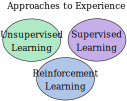
\includegraphics[height=5cm]{figs/experience.png}
    \end{center}

\end{frame}


\begin{frame}

    \frametitle{General Approach to Supervised Learning}

    \begin{itemize}
        \item Acquire the data.
        \item Prepocess the data.
        \item Split the data.
        \item Develop the Network Architecture.
        \item Select training hyperparamters.
        \item Train the network.
        \item Repeat steps 4 - 6 until satisfactory performance.
    \end{itemize}

\end{frame}

\begin{frame}

    \frametitle{Acquire the Data}

    \begin{itemize}
        \item Can be a tedious and time consuming process.
        \item In engineering this is generally not the case.
        \item Critical to understand the problem you are trying to solve.
    \end{itemize}

    \begin{center}
        \includegraphics[height=4cm]{figs/mnist_examples.png}
    \end{center}

\end{frame}


\begin{frame}

    \frametitle{Prepare the Data}

    \begin{itemize}
        \item Clean the data
        \item Normalize the data
    \end{itemize}

\end{frame}

\end{document}